\documentclass{standalone}
\usepackage{tikz}
\usetikzlibrary{patterns, positioning}

\begin{document}
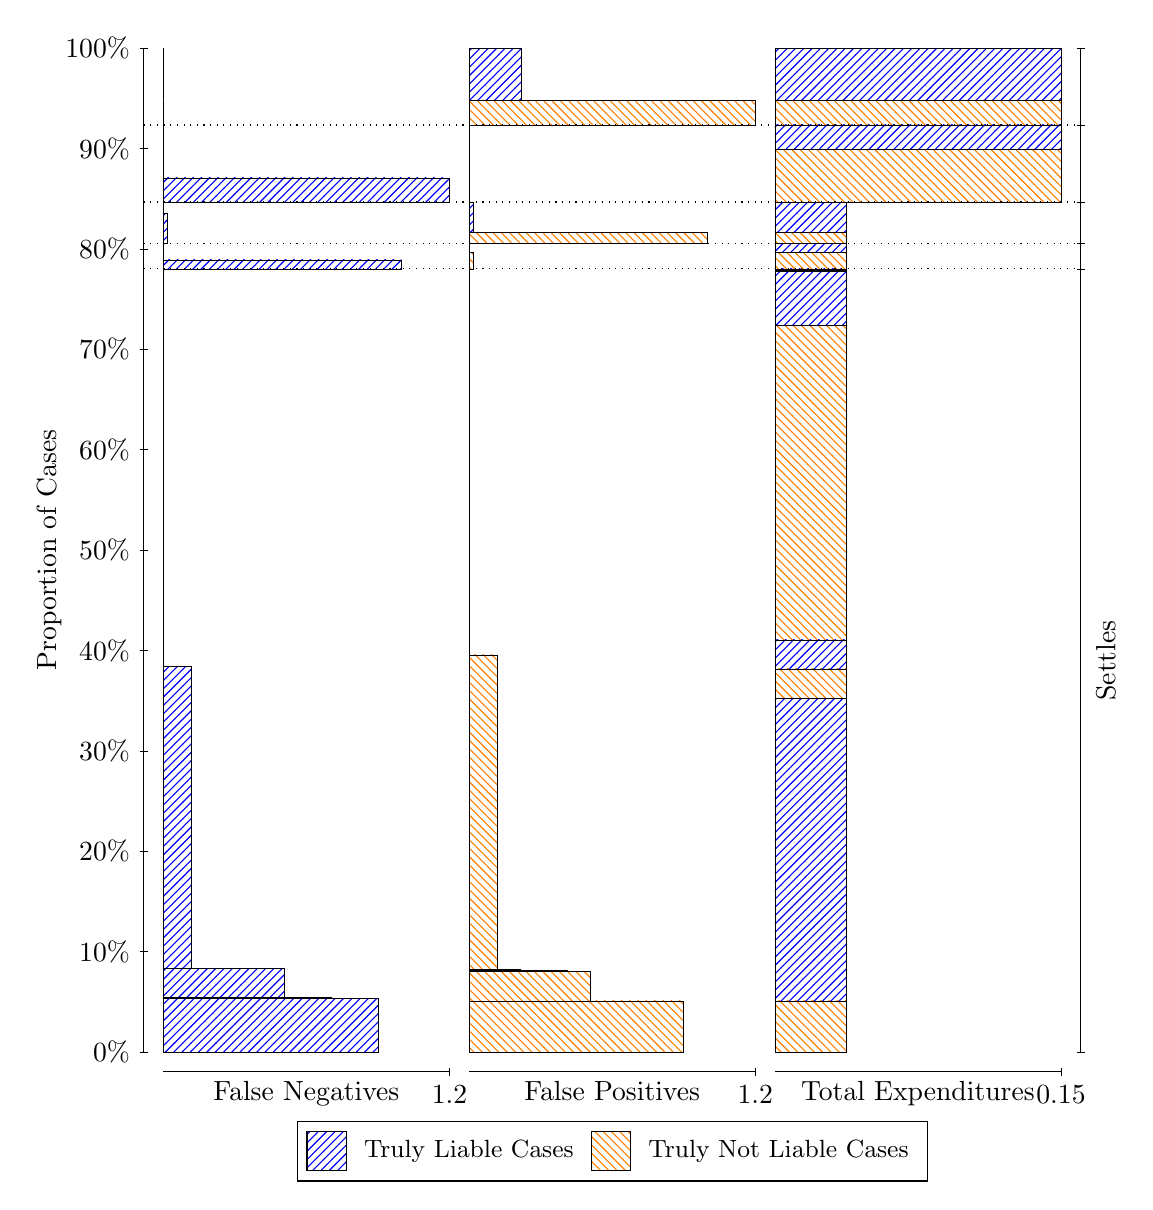
\begin{tikzpicture}
\draw[black, very thin] (1.5,1.75) -- (1.5,14.5);
\node[rotate=90, anchor=center] at (0.3, 8.125) {Proportion of Cases};
\draw[black, very thin] (1.45,1.75) -- (1.55,1.75);
\node[anchor=east] at (1.45, 1.75) {0\%};
\draw[black, very thin] (1.45,3.025) -- (1.55,3.025);
\node[anchor=east] at (1.45, 3.025) {10\%};
\draw[black, very thin] (1.45,4.3) -- (1.55,4.3);
\node[anchor=east] at (1.45, 4.3) {20\%};
\draw[black, very thin] (1.45,5.575) -- (1.55,5.575);
\node[anchor=east] at (1.45, 5.575) {30\%};
\draw[black, very thin] (1.45,6.85) -- (1.55,6.85);
\node[anchor=east] at (1.45, 6.85) {40\%};
\draw[black, very thin] (1.45,8.125) -- (1.55,8.125);
\node[anchor=east] at (1.45, 8.125) {50\%};
\draw[black, very thin] (1.45,9.4) -- (1.55,9.4);
\node[anchor=east] at (1.45, 9.4) {60\%};
\draw[black, very thin] (1.45,10.675) -- (1.55,10.675);
\node[anchor=east] at (1.45, 10.675) {70\%};
\draw[black, very thin] (1.45,11.95) -- (1.55,11.95);
\node[anchor=east] at (1.45, 11.95) {80\%};
\draw[black, very thin] (1.45,13.225) -- (1.55,13.225);
\node[anchor=east] at (1.45, 13.225) {90\%};
\draw[black, very thin] (1.45,14.5) -- (1.55,14.5);
\node[anchor=east] at (1.45, 14.5) {100\%};

\draw[black, very thin] (13.4,1.75) -- (13.4,14.5);
\draw[black, very thin] (13.35,1.75) -- (13.45,1.75);
\node[anchor=west] at (13.35, 1.75) {};
\draw[black, very thin] (13.35,11.696) -- (13.45,11.696);
\node[anchor=west] at (13.35, 11.696) {};
\draw[black, very thin] (13.35,12.02) -- (13.45,12.02);
\node[anchor=west] at (13.35, 12.02) {};
\draw[black, very thin] (13.35,12.544) -- (13.45,12.544);
\node[anchor=west] at (13.35, 12.544) {};
\draw[black, very thin] (13.35,13.523) -- (13.45,13.523);
\node[anchor=west] at (13.35, 13.523) {};
\draw[black, very thin] (13.35,14.5) -- (13.45,14.5);
\node[anchor=west] at (13.35, 14.5) {};

\draw[black, very thin, pattern color=blue, pattern=north east lines] (1.75,1.75) rectangle (4.475,2.4271);
\draw[black, very thin, pattern color=blue, pattern=north east lines] (1.75,2.4271) rectangle (4.1784,2.4329);
\draw[black, very thin, pattern color=blue, pattern=north east lines] (1.75,2.4329) rectangle (3.8818,2.4389);
\draw[black, very thin, pattern color=blue, pattern=north east lines] (1.75,2.4389) rectangle (3.5852,2.445);
\draw[black, very thin, pattern color=blue, pattern=north east lines] (1.75,2.445) rectangle (3.2886,2.8132);
\draw[black, very thin, pattern color=blue, pattern=north east lines] (1.75,2.8132) rectangle (2.1022,6.6515);
\draw[black, very thin, pattern color=orange, pattern=north west lines] (1.75,6.6515) rectangle (1.75,11.696);
\draw[black, very thin, pattern color=blue, pattern=north east lines] (1.75,11.696) rectangle (4.7716,11.809);
\draw[black, very thin, pattern color=orange, pattern=north west lines] (1.75,11.809) rectangle (1.75,12.02);
\draw[black, very thin, pattern color=blue, pattern=north east lines] (1.75,12.02) rectangle (1.8056,12.403);
\draw[black, very thin, pattern color=orange, pattern=north west lines] (1.75,12.403) rectangle (1.75,12.544);
\draw[black, very thin, pattern color=blue, pattern=north east lines] (1.75,12.544) rectangle (5.3833,12.852);
\draw[black, very thin, pattern color=orange, pattern=north west lines] (1.75,12.852) rectangle (1.75,13.523);
\draw[black, very thin, pattern color=orange, pattern=north west lines] (1.75,13.523) rectangle (1.75,13.832);
\draw[black, very thin, pattern color=blue, pattern=north east lines] (1.75,13.832) rectangle (1.75,14.5);
\draw[black, very thin, pattern color=orange, pattern=north west lines] (5.6333,1.75) rectangle (8.3583,2.3994);
\draw[black, very thin, pattern color=orange, pattern=north west lines] (5.6333,2.3994) rectangle (7.1719,2.778);
\draw[black, very thin, pattern color=orange, pattern=north west lines] (5.6333,2.778) rectangle (6.8753,2.7842);
\draw[black, very thin, pattern color=orange, pattern=north west lines] (5.6333,2.7842) rectangle (6.5787,2.7902);
\draw[black, very thin, pattern color=orange, pattern=north west lines] (5.6333,2.7902) rectangle (6.2821,2.7962);
\draw[black, very thin, pattern color=orange, pattern=north west lines] (5.6333,2.7962) rectangle (5.9855,6.7941);
\draw[black, very thin, pattern color=blue, pattern=north east lines] (5.6333,6.7941) rectangle (5.6333,11.696);
\draw[black, very thin, pattern color=orange, pattern=north west lines] (5.6333,11.696) rectangle (5.6889,11.906);
\draw[black, very thin, pattern color=blue, pattern=north east lines] (5.6333,11.906) rectangle (5.6333,12.02);
\draw[black, very thin, pattern color=orange, pattern=north west lines] (5.6333,12.02) rectangle (8.6549,12.16);
\draw[black, very thin, pattern color=blue, pattern=north east lines] (5.6333,12.16) rectangle (5.6889,12.544);
\draw[black, very thin, pattern color=orange, pattern=north west lines] (5.6333,12.544) rectangle (5.6333,13.215);
\draw[black, very thin, pattern color=blue, pattern=north east lines] (5.6333,13.215) rectangle (5.6333,13.523);
\draw[black, very thin, pattern color=orange, pattern=north west lines] (5.6333,13.523) rectangle (9.2667,13.832);
\draw[black, very thin, pattern color=blue, pattern=north east lines] (5.6333,13.832) rectangle (6.3007,14.5);
\draw[black, very thin, pattern color=orange, pattern=north west lines] (9.5167,1.75) rectangle (10.425,2.3994);
\draw[black, very thin, pattern color=blue, pattern=north east lines] (9.5167,2.3994) rectangle (10.425,6.2376);
\draw[black, very thin, pattern color=orange, pattern=north west lines] (9.5167,6.2376) rectangle (10.425,6.6163);
\draw[black, very thin, pattern color=blue, pattern=north east lines] (9.5167,6.6163) rectangle (10.425,6.9846);
\draw[black, very thin, pattern color=orange, pattern=north west lines] (9.5167,6.9846) rectangle (10.425,10.982);
\draw[black, very thin, pattern color=blue, pattern=north east lines] (9.5167,10.982) rectangle (10.425,11.66);
\draw[black, very thin, pattern color=orange, pattern=north west lines] (9.5167,11.66) rectangle (10.425,11.678);
\draw[black, very thin, pattern color=blue, pattern=north east lines] (9.5167,11.678) rectangle (10.425,11.696);
\draw[black, very thin, pattern color=orange, pattern=north west lines] (9.5167,11.696) rectangle (10.425,11.906);
\draw[black, very thin, pattern color=blue, pattern=north east lines] (9.5167,11.906) rectangle (10.425,12.02);
\draw[black, very thin, pattern color=orange, pattern=north west lines] (9.5167,12.02) rectangle (10.425,12.16);
\draw[black, very thin, pattern color=blue, pattern=north east lines] (9.5167,12.16) rectangle (10.425,12.544);
\draw[black, very thin, pattern color=orange, pattern=north west lines] (9.5167,12.544) rectangle (13.15,13.215);
\draw[black, very thin, pattern color=blue, pattern=north east lines] (9.5167,13.215) rectangle (13.15,13.523);
\draw[black, very thin, pattern color=orange, pattern=north west lines] (9.5167,13.523) rectangle (13.15,13.832);
\draw[black, very thin, pattern color=blue, pattern=north east lines] (9.5167,13.832) rectangle (13.15,14.5);
\draw[black, dotted] (1.5,11.696) -- (13.4,11.696);
\draw[black, dotted] (1.5,12.02) -- (13.4,12.02);
\draw[black, dotted] (1.5,12.544) -- (13.4,12.544);
\draw[black, dotted] (1.5,13.523) -- (13.4,13.523);
\draw[black, very thin] (1.75,1.5) -- (5.3833,1.5);
\node[anchor=north] at (3.5667, 1.5) {False Negatives};
\draw[black, very thin] (5.3833,1.45) -- (5.3833,1.55);
\node[anchor=north] at (5.3833, 1.45) {1.2};

\draw[black, very thin] (5.6333,1.5) -- (9.2667,1.5);
\node[anchor=north] at (7.45, 1.5) {False Positives};
\draw[black, very thin] (9.2667,1.45) -- (9.2667,1.55);
\node[anchor=north] at (9.2667, 1.45) {1.2};

\draw[black, very thin] (9.5167,1.5) -- (13.15,1.5);
\node[anchor=north] at (11.333, 1.5) {Total Expenditures};
\draw[black, very thin] (13.15,1.45) -- (13.15,1.55);
\node[anchor=north] at (13.15, 1.45) {0.15};

\node[black, centered, rotate=90] at (13.72, 6.7228) {Settles};





\draw (7.449999999999999,1.5) node[draw=none] (baseCoordinate) {};
\begin{scope}[align=center]
        \matrix[scale=0.5, draw=black, below=0.5cm of baseCoordinate, nodes={draw}, column sep=0.1cm]{
            \node[rectangle, draw, minimum width=0.5cm, minimum height=0.5cm, pattern=north east lines, pattern color=blue] {}; &
            \node[draw=none, font=\small] (B) {Truly Liable Cases}; &
            \node[rectangle, draw, minimum width=0.5cm, minimum height=0.5cm, pattern=north west lines, pattern color=orange] {}; &
            \node[draw=none, font=\small] (B) {Truly Not Liable Cases}; \\
            };
\end{scope}

\end{tikzpicture}
\end{document}